%%%%%%%%%%%%%%%%%%%%%%%%%%%%%%%%%%%%%%%%%
% Simple Sectioned Essay Template
% LaTeX Template
%
% This template has been downloaded from:
% http://www.latextemplates.com
%
% Note:
% The \lipsum[#] commands throughout this template generate dummy text
% to fill the template out. These commands should all be removed when 
% writing essay content.
%
%%%%%%%%%%%%%%%%%%%%%%%%%%%%%%%%%%%%%%%%%

%----------------------------------------------------------------------------------------
%	PACKAGES AND OTHER DOCUMENT CONFIGURATIONS
%----------------------------------------------------------------------------------------
%
\documentclass[12pt]{article} % Default font size is 12pt, it can be changed here

\renewcommand{\familydefault}{\sfdefault} % Standardfont �ndern auf Sans Se rif (bny)

\usepackage[left=3cm,right=2.5cm,top=2.5cm,bottom=3cm]{geometry} % Required to change the page size to A4
% manuelle Seitenr�nder eingesetzt durch bny einfach alles inkl. [] wieder l�schen, 09.04.2016
\geometry{a4paper} % Set the page size to be A4 as opposed to the default US Letter

\usepackage[utf8x]{inputenc}
\usepackage[german]{babel} % Sprache umschalten /hat funktioniert bis auf Authors, bny 13.04.2016
\usepackage{graphicx} % Required for including pictures
\usepackage{graphics} % M�glichkeit Bilder im Textfluss einzubinden - bny / 09.04.2016
\usepackage{float} % Allows putting an [H] in \begin{figure} to specify the exact location of the figure
\usepackage{wrapfig} % Allows in-line images such as the example fish picture
\usepackage[dvipsnames]{xcolor} % von bny hinzugef�gt
\usepackage{paralist} % Aufz�hlung mit weniger Abstand - bny
\usepackage[bookmarksopen=true,colorlinks,linkcolor = black]{hyperref} % Hinzugef�gt am 21.04.2016 - bny
\usepackage{adjustbox} % Bild/Text ausrichten; hinzugef�gt am 21.04.2016, bny
\usepackage{eurosym}
\usepackage{xcolor} % f�r Textbox mit Farbhintergrund, bny 09.11.2018
\usepackage{mdframed} % f�r Textbox mit Farbhintergrund, bny 09.11.2018

\linespread{1.2} % Line spacing
%\setlength\parindent{0pt} % Uncomment to remove all indentation from paragraphs
\graphicspath{{Pictures/}} % Specifies the directory where pictures are stored
\setlength{\parindent}{0pt} % Neue Abs�tze nicht einr�cken - bny 09.04.2016

\newcommand{\HRule}{\rule{\linewidth}{0.5mm}} % Defines a new command for the horizontal lines, change thickness here
\newcommand{\col}[1]{\textbf{\textcolor[rgb]{0.4392157,0.1882353,0.627451}{#1}}}


%----------------------------------------------------------------------------------------
%	BEGIN DOCUMENT
%----------------------------------------------------------------------------------------

\begin{document}

%----------------------------------------------------------------------------------------
%	TITLE PAGE
%----------------------------------------------------------------------------------------

\begin{titlepage}

\begin{flushright}

\includegraphics[width=0.6\linewidth]{LogoPG_RBS_Verbindet.jpg}
\end{flushright}

\begin{flushright}

\includegraphics[width=0.2\linewidth]{1_RBSLogo}
\end{flushright}

% \begin{figure}[t] % Example image
% \flushright  % rechtsbuendig
% 
\includegraphics[width=.6\linewidth]{LogoPG_RBS_Verbindet.jpg} \newline 
\includegraphics[width=0.2\linewidth]{1_RBSLogo}
% \end{figure}

\vspace*{1cm}

\center

\HRule \\[0.4cm]
{ \huge \bfseries CUBE ProjectAssistant - Reprodruck}\\[0.4cm] % Title of your document
\HRule \\[1.5cm]

\textsf{\Large Spezialanleitung}\\[0.5cm] % Major heading such as course name
\textsf{\large Version 2.12 / 20.12.2018}\\[0.5cm] % Minor heading such as course title

\vspace*{1.5cm}

\flushleft\textbf{ Impressum}
\rule{\textwidth}{1pt}
% \begin{flushright}
% \begin{flushleft}

% \end{flushleft}
% \end{flushright}
\vspace{\baselineskip}

\begin{tabular}{lp{12cm}}
Auftragsnummer & BE.N.\\
Auftraggeber & .\\
Datum & 20.12.2018\\
Version & 2.12\\
Autor & Benjamin Nyffenegger\\
% Freigabe & Markus Schafroth\\
Verteilen & .\\
Datei & .\\
Seitenzahl & 12 \\
Copyright & \copyright{ Emch+Berger AG Bern}\\
\end{tabular}

\vspace*{1.2cm}

\begin{flushright}
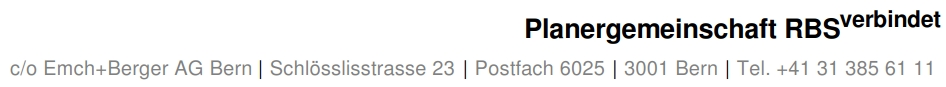
\includegraphics[width=1\linewidth]{Pictures/Planergemeinschaft.jpg}
\end{flushright}

\vfill % Fill the rest of the page with whitespace

\end{titlepage}

%----------------------------------------------------------------------------------------
%	TABLE OF CONTENTS
%----------------------------------------------------------------------------------------

\tableofcontents % Include a table of contents

% \newpage % Begins the essay on a new page instead of on the same page as the table of contents 

%----------------------------------------------------------------------------------------
%	Eingebundene Kapitel
%----------------------------------------------------------------------------------------
% Achtung, werden Kapitel ein-/ausgeblendet -> in Titelseite Seiteanzahl anpassen


\section{Auswahl von Plänen / Dokumenten für den Plandruck}
Klicken Sie im Hauptmenü auf 'Dokumentenablage' und den Unterpunkt 'Dokumente'. Die Übersicht der Dokumente erscheint:

\begin{figure}[H]
\center{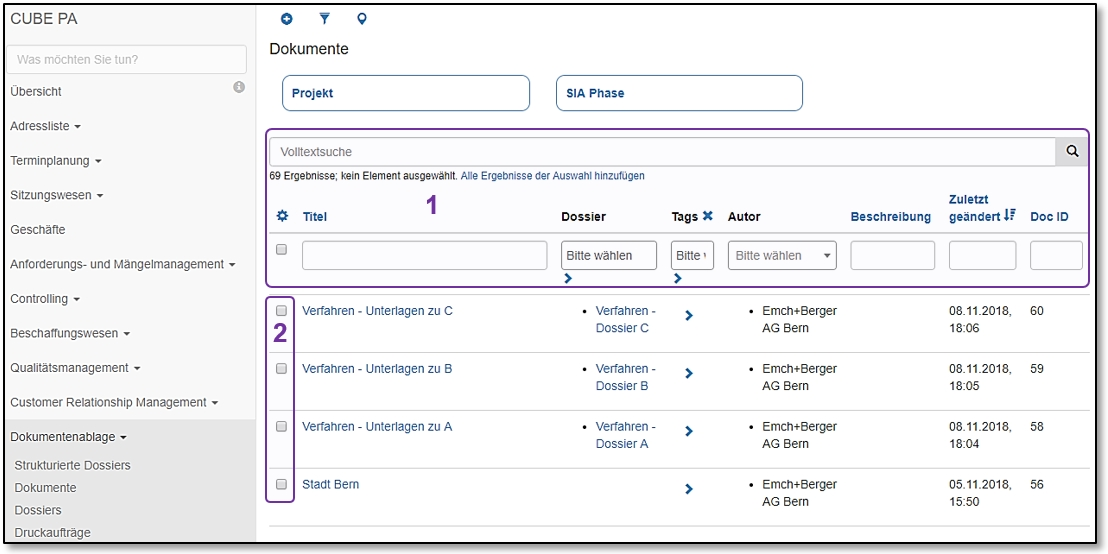
\includegraphics[width=1\linewidth]{../chapters/11_Dokumentenablage/pictures/docrep_DokUebersicht.jpg}}
\caption{Übersicht der Dokumente}
% \label{fig:speciation}
\end{figure}

Suchen Sie mit den Filterfeldern und der Volltextsuche \col{(1)} nach den gewünschten Dokumenten. Sobald Sie ein Suchwort eingegeben haben, beginnt die Suche und das Resultat wird umgehend angezeigt. Wählen Sie mit den Checkboxen \col{(2)} alle benötigten Dokumente und Pläne für den Versand aus. Die Auswahl wird im Dokumentenkorb (analog zu einem Warenkorb) zusammengefasst.

\vspace{\baselineskip}

Sobald Sie ein Dokument ausgewählt und damit in den Warenkorb gelegt haben, werden Ihnen oben im Browserfenster die möglichen Optionen angezeigt:

\begin{figure}[H]
\center{
\includegraphics[width=1\linewidth]{../chapters/11_Dokumentenablage/pictures/dkorb_wOptionen.jpg}}
\caption{Optionen}
% \label{fig:speciation}
\end{figure}

\textbf{Hinweis:} Die Anzahl an Optionen kann je nach Auswahl variieren. Wurde nur ein Dokument / Plan ausgewählt, haben Sie mehr Optionen. Wurde mit einem Dokument auch ein Link ausgewählt, können Sie nur wenige Optionen anwählen.

\begin{wrapfigure}[11]{l}{2.8cm}
\vspace{-15pt}
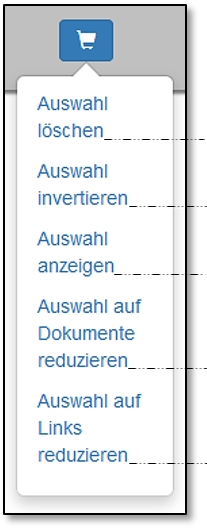
\includegraphics[height=70mm]{../y_SpezDokus/chapters/11_Dokumentenablage/pictures/11-dkorb_Auswahl.jpg}
% \caption{Status ändern}
\end{wrapfigure}
Klicken Sie auf den Dokumentenkorb 
\includegraphics[height=12pt]{/Icons/dk_korb_b.jpg}, um weitere Optionen rund um die Dokumentenauswahl zu sehen. Die angezeigten Optionen sind abhängig von der Anzahl und der Art der ausgewählten Dokumenten oder Links:

- \mbox{'Auswahl löschen' löscht gesamter Inhalt des Dokumentenkorbs.}\\
- Sie können die 'Auswahl invertieren'.\\
- Klick auf 'Auswahl anzeigen' führt sämtlich Dokumente und Links im Dokumentenkorb auf.\\
- Haben Sie Dokumente und Links markiert, kann die Selektion auf Dokumente oder Links reduzieren werden.\\

\vspace{\baselineskip}


\includegraphics[height=12pt]{/Icons/dk_lupe.jpg} : Sie gelangen in den Ansichtsmodus des Dokumentes\\

\includegraphics[height=12pt]{/Icons/dk_bearb.jpg} : Sie gelangen in den Bearbeitungsmodus des Dokumentes\\

\includegraphics[height=12pt]{/Icons/dk_flag_b.jpg} : Damit markieren Sie ein Dokument / Link als Favorit. In der Folge erscheint das Dokument / der Link in Ihrer persönlichen Projektübersicht\\

\includegraphics[height=12pt]{/Icons/dk_nadel.jpg} : Öffnet die Karte und zeigt Ihnen wo das Dokument verortet ist\\

\includegraphics[height=12pt]{/Icons/dk_download.jpg} : Laden sie sämtliche ausgewählten Dokumente als ZIP-File herunter (Ist ein Dokument ausgewählt, wird es im effektiven Format heruntergeladen)\\

\includegraphics[height=12pt]{/Icons/dk_senden.jpg} : Versenden Sie Dokumente per Attachement oder per Link\\

\includegraphics[height=12pt]{/Icons/dk_drucken.jpg} : \textbf{Die ausgewählten Dokumente werden an ein ReproZentrum verschickt. Die Details werden unten in dieser Anleitung ausgeführt}\\

\includegraphics[height=12pt]{/Icons/dk_auschecken.jpg} : Das ausgewählte Dokument wird für die Bearbeitung ausgecheckt und steht den anderen Benutzern während dieser Aktion für die Bearbeitung nicht zur Verfügung (Herunterladen ist jedoch möglich)\\

\includegraphics[height=12pt]{/Icons/A_Benachrichtigungsregel.jpg} : Für das ausgewählte Dokument kann eine Benachrichtigungsregel eingerichtet werden. Bei Veränderungen erhalten Sie eine Email.\\

\vspace{\baselineskip}

\textbf{Hinweis}: Die Details der oben beschrieben Funktionen finden Sie im CUBE Project Assistant Haupthandbuch.

\vspace{\baselineskip}

\section{Druckaufträge an Reprozentren senden}
% Neues Kapitel

Pläne können direkt aus der Dokumentenablage an Reprozentren zur Direktauslieferung von geplotteten Plänen gesendet werden. Mehrere Pläne können im Rahmen einer einzigen Bestellung an mehrere Empfänger verschickt werden, wobei die Ausführung (Anzahl Exemplare, Druck-/elektronische Kopie) pro Empfänger separat festgelegt werden kann.

\vspace{\baselineskip}

Für das Versenden von Plänen via Reprozentren gehen Sie wie folgt vor: Wählen Sie wie oben beschrieben sämtliche benötigten Dokumente / Pläne aus und legen Sie diese in den Dokumentenkorb. In Ihrem Dokumentenkorb sehen Sie nun alle ausgewählten Dokumente. Haben Sie zu viele Dokumente ausgewählt / markiert, können Sie bei diesen Dokumenten die Markierung wieder herausnehmen 
\includegraphics[height=12pt]{/Icons/checkbox_markiert.jpg} - 
\includegraphics[height=12pt]{/Icons/checkbox_leer.jpg} und den Warenkorb entsprechend anpassen. Sind alle Dokumente / Pläne beisammen, klicken Sie im Dokumentenkorb auf das Drucker-Symbol 
\includegraphics[height=12pt]{/Icons/dk_drucken.jpg}. Es öffnet sich folgendes Fenster:

\begin{figure}[H]
\center{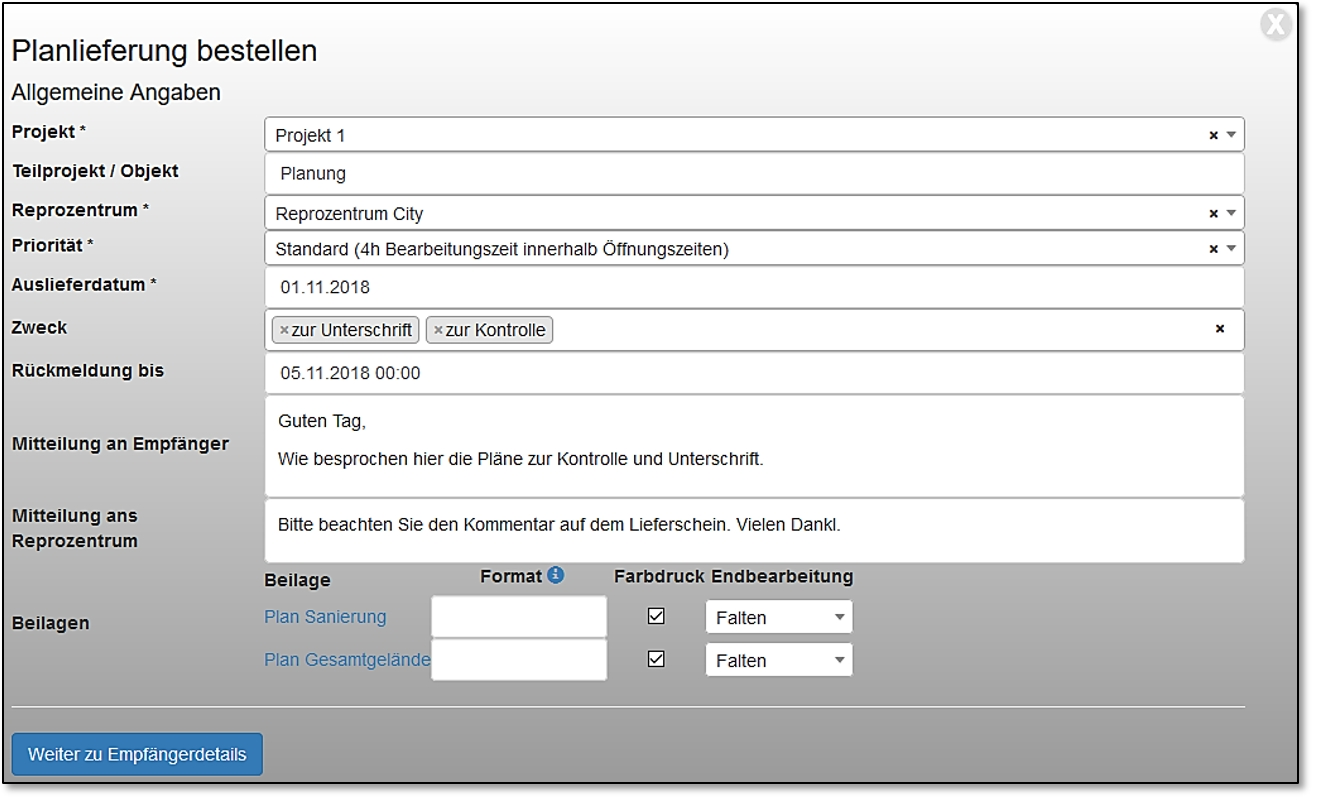
\includegraphics[width=1\linewidth]{../chapters/11_Dokumentenablage/pictures/11-dkorb_ReproDialog1.jpg}}
\caption{Dialogfenster 'Allgemeine Angaben' für die Planlieferung}
% \label{fig:speciation}
\end{figure}

Wählen oder ergänzen Sie folgende Felder:

\textbf{Projekt:} Dies ist ein Pflichtfeld. Wählen Sie in der vordefinierten Liste der eingetragenen Projekten das entsprechende Projekt aus. \\
\textbf{Teilprojekt / Objekt:} Mittels Freitext können Sie hier ergänzende Informationen zum Projekt hinterlegen. \\
\textbf{Reprozentrum:} Dies ist ein Pflichtfeld. Sämtliche in den Voreinstellungen (Konfiguration) hinterlegten Reprozentren können Sie hier für die Planlieferung auswählen. \\
\textbf{Priorität:} Dies ist ein Pflichtfeld. Sie können zwischen drei verschiedenen Prioritäten auswählen:
\begin{figure}[H]
\center{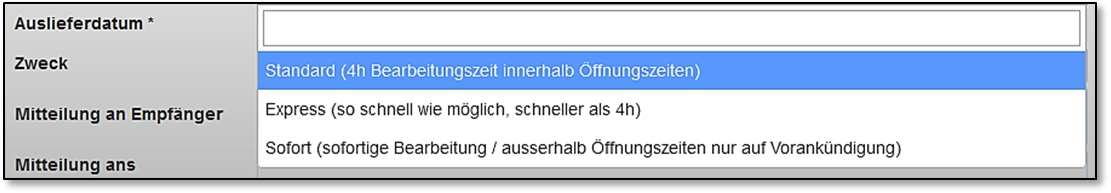
\includegraphics[width=1\linewidth]{../chapters/11_Dokumentenablage/pictures/11-dkorb_ReproPrio}}
\caption{Prioritätenauswahl für Planlieferung}
% \label{fig:speciation}
\end{figure}
Beachten Sie, dass die Auslieferung auch abhängig ist von der Bestellzeit. Für Detailklärung kontaktieren Sie die zuständigen Stellen. \\
\textbf{Auslieferungsdatum:} Dies ist ein Pflichtfeld. Das Auslieferungsdatum wird automatisch in Abhängigkeit der gewählten Priorität gesetzt und kann nachträglich geändert werden. \\
\textbf{Zweck:} Sie können hier aus einer Liste vordefinierter Angaben einen oder mehrere Zweck(e) auswählen, welche/r dann auf dem Lieferschein für die Empfänger erscheint.
\begin{figure}[H]
\center{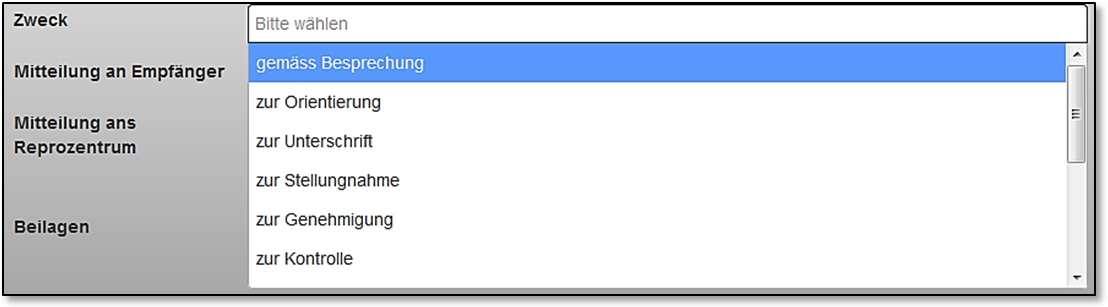
\includegraphics[width=1\linewidth]{../chapters/11_Dokumentenablage/pictures/11-dkorb_ReproZweck}}
\caption{Zweckangabe für den Lieferschein}
% \label{fig:speciation}
\end{figure}
\textbf{Rückmeldung bis} Terminieren Sie den 'Zweck' und setzen Sie das gewünschte Datum. \\
\textbf{Mitteilung an Empfänger:} Hier können Sie mittels Freitext die nötigen Angaben für den/die Empfänger eingeben. \\
\textbf{Mitteilung an das Reprozentrum:} Diese Angaben sind nach Abschluss der Planbestellung für das Reprozentrum sichtbar. \\
\textbf{Beilagen:} Pro Dokument, welches im Dokumentenkorb war und nun für die Planlieferung zur Verfügung steht, können Sie Detailangaben vornehmen. Mit Klick auf den blauen Dokumententitel können Sie das Dokument / den Plan nochmals öffnen oder auf Ihrem Computer abspeichern.
In der Regel wird die Grösse des Plans in Abhängigkeit des PDF's bestimmt. Sie haben jedoch die Möglichkeit hier Einfluss zu nehmen und Anpassungen des Format dem Reprozentrum mitzuteilen. Zudem können Sie pro Dokument / Plan auswählen, ob dieser in Farbe oder s/w ausgedruckt und geliefert werden soll. Sie können abschliessend noch definieren, in welcher Form / Endbearbeitung der Plan auf die Baustelle oder in ein Büro geliefert werden soll (Falten, Heften, Heftstreifen, Nach Absprache, Rollen, Spiralbinden, Thermobindung).
Haben Sie alle nötigen Angaben gemacht, klicken Sie auf 'Weiter zu Empfängerdetails' um zu den 'Empfängerdetails' zu gelangen:

\begin{figure}[H]
\center{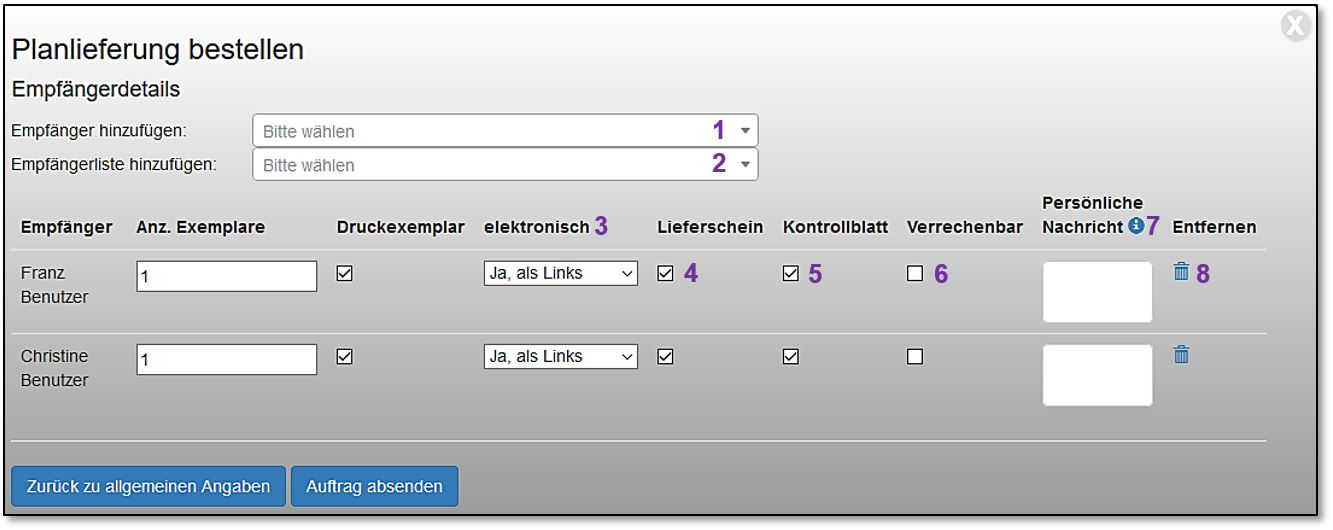
\includegraphics[width=1\linewidth]{../chapters/11_Dokumentenablage/pictures/11-dkorb_ReproDialog2.jpg}}
\caption{Dialogfenster 'Empfängerdetails' für die Planlieferung}
% \label{fig:speciation}
\end{figure}

Hier können Sie einen oder mehrere Empfänger auswählen \col{(1)} oder eine vordefinierte Empfängerliste wählen \col{(2)}. Gehen Sie wie folgt vor: aus der Dropdownliste 'Empfänger hinzufügen' wählen Sie die gewünschte Person aus. Wiederholen Sie diesen Schritt mit weiteren benötigten Empfängern. So bald Sie einen Empfänger aus der Liste ausgewählt haben, erscheint dieser unten im Dialogfenster. Sie können nun noch weitere Einstellungen vornehmen, wie zum Beispiel wie viele Exemplare pro Empfänger benötigt werden und ob der / die Empfänger die Pläne ausgedruckt (Druckexemplar) oder als PDF/Dokument per E-Mail zugestellt benötigt / benötigen (elektronisch). \\

\begin{wrapfigure}[4]{r}{5cm}   % [x] Wie manche Zeile soll sich um die Grafik "brechen"
  \vspace{-30pt}      % Grundwert war 20; mit 30 schön oben beim Text ausgerichtet
  \begin{center}
    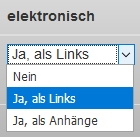
\includegraphics[width=1\linewidth]{../chapters/11_Dokumentenablage/pictures/repro_elektronisch.jpg}
  \end{center}
  \vspace{-20pt}
%  \caption{Zusammenfassung im Excelexport}
  \vspace{-10pt}
\end{wrapfigure}
Sollen die Pläne/Dokumente 'elektronisch' \col{(3)} verteilt werden, können Sie aus nebenstehenden Optionen auswählen:\\
Wird 'Ja, als Links (ohne Login)' gewählt, erhält der Empfänger einen Dokumentenlink, welcher 30 Tage gültig ist und ohne CUBE-Login abgerufen werden kann.

\vspace{.5cm} 

Wird ein Lieferschein benötigt, kann dies pro Person definiert werden \col{(4)}. Sollen Rückmeldung der Pläne/Dokumente erfolgen, kann ein Kontrollblatt generiert und verschickt werden \col{(5)}. Sind die Drucklieferungen verrechenbar wird das Häkchen entsprechend gesetzt \col{(6)}. Haben Sie mehrere Empfänger und soll für bestimmte Empfänger eine persönliche Nachricht (anstelle der allgemeinen Nachricht) verschickt werden (E-Mail / Lieferschein), können Sie die gewünschte individuelle Nachricht unter 'Persönliche Nachricht' \col{(7)} eintragen. Klicken Sie auf das 
\includegraphics[height=12pt]{/Icons/Info_blau.jpg}. \col{(7)}, erhalten Sie die entsprechende Information.\\
Mit dem Mülltonnensymbol 
\includegraphics[height=12pt]{/Icons/Muelltonne.jpg} \col{(8)} können Sie die ausgewählten Empfänger wieder löschen. Werden mittels obiger Dropdownliste 'Empfänger hinzufügen' \col{(1)} Empfänger ausgewählt, welche bereits unten in der Liste stehen, erscheint folgende Meldung:

\begin{figure}[H]
\center{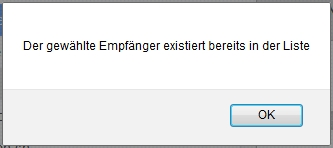
\includegraphics[width=.5\linewidth]{../chapters/11_Dokumentenablage/pictures/11-dkorb_Meldung_doppeltePerson.jpg}}
\caption{Meldung: Empfänger existiert bereits}
% \label{fig:speciation}
\end{figure}

\textbf{Hinweis:} Die Verteilerliste im Email erscheint nur, wenn 'kein Lieferschein' ausgewählt wurde \col{(4)}.

\vspace{\baselineskip}

Müssen Sie nochmals bei den 'Allgemeinen Angaben' Änderungen vornehmen oder diese kontrollieren, können Sie mittels Klick auf 'Zurück zu allgemeinen Angaben' wieder zu diesen Angaben gelangen. Ist alles in Ordnung und wollen Sie die Pläne wie nun definiert bestellen, klicken Sie auf 'Auftrag absenden'. Die entsprechenden Emails (Bestätigung, Bestellung, elektronische Lieferung) werden verschickt und CUBE PA öffnet in der Dokumentenablage im Ansichtsmodus den Lieferschein. Das Reprozentrum erhält den Auftrag per Email mit einem Link in den CUBE PA. Dort können sie den Auftrag bearbeiten und die benötigten Dokumente / Pläne herunterladen. Wurde der Auftrag durch das Reprozentrum bearbeitet, resp. ausgelöst, wird durch das Reprozentrum die Bestellung als 'abgeschlossen' markiert. Dies wird dem Besteller so auch protokolliert.

\vspace{\baselineskip}

Wurde eine Bestellung ausgelöst, wird diese beim Besteller (Bearbeiter des CUBE PA) in der Übersicht angezeigt. Wurde durch das Reprozentrum wie oben beschrieben der Auftrag / die Bestellung als 'abgeschlossen' markiert, wird dies ebenfalls in der Übersicht angezeigt.

\vspace{\baselineskip}

\textbf{Wichtiger Hinweis:} Wird während den Eingaben in oben beschriebenen Formularen auf das Kreuzchen \includegraphics[height=12pt]{/Icons/X_BUtton.jpg} (rechts oben) geklickt, verlieren Sie sämtliche Einstellungen / Eingaben. Die Dokumente / Pläne bleiben noch im Dokumentenkorb und Sie können wieder mit einem neuen Auftrag beginnen.

\vspace{\baselineskip}

\clearpage
\textbf{Excel Kontrollblatt}\\

\begin{figure}[H]
\center{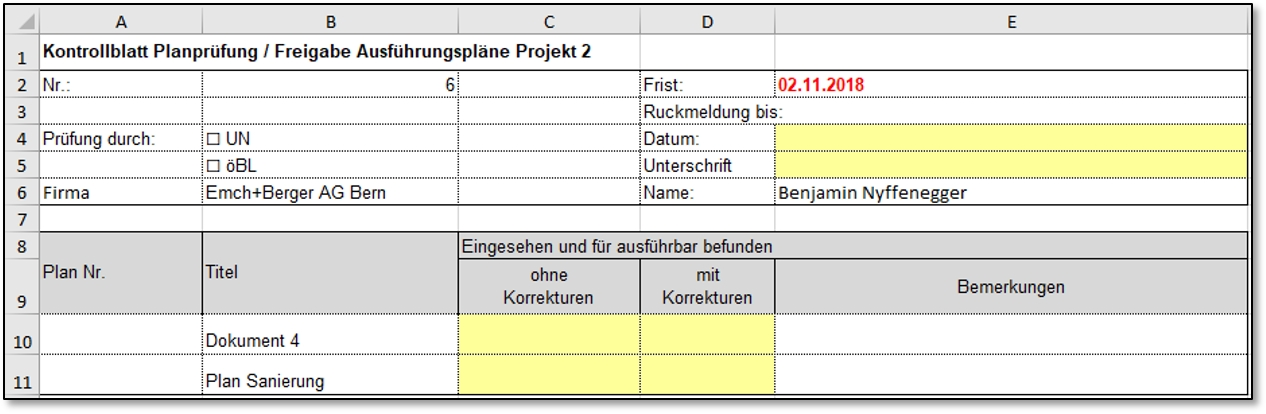
\includegraphics[width=1\linewidth]{../chapters/11_Dokumentenablage/pictures/repro_Kontrollblatt.jpg}}
\caption{Excel Kontrollblatt}
% \label{fig:speciation}
\end{figure}

Wie oben beschrieben, können Sie pro Person und Auftrag festlegen, ob ein Kontrollblatt erstellt werden soll. Dieses dient dazu, Rückmeldungen hinsichtlich den versendeten Plänen / Dokumenten notieren zu können. Beispielsweise werden Korrekturen oder auch 'Dokumentfreigaben' mittels dem Kontrollblatt festgehalten und zurückgemeldet.

\pagebreak
\textbf{Die Druckaufträge in der Übersicht:}\\

\begin{wrapfigure}[5]{l}{6.5cm}   % [x] Wie manche Zeile soll sich um die Grafik "brechen"
  \vspace{-35pt}      % Grundwert war 20; mit 30 schön oben beim Text ausgerichtet
  \begin{center}
    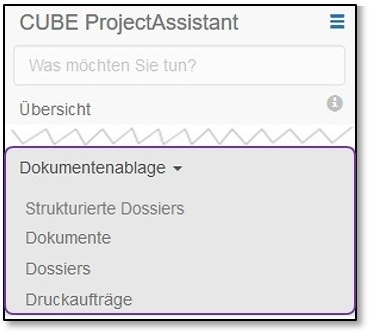
\includegraphics[width=1\linewidth]{../chapters/11_Dokumentenablage/pictures/11_Menu_Dokumentenablage_s.jpg}
  \end{center}
  \vspace{-20pt}
  \caption{Druckaufträge aufrufen}
  \vspace{-10pt}
\end{wrapfigure}

Wählen Sie im Menü links den Menüpunkt 'Dokumentenablage' und den Unterpunkt 'Druckaufträge'. Sie gelangen zur Übersicht der Druckaufträge, bei welcher Sie wie gewohnt nach Einträgen suchen und filtern können.

\vspace{4cm} 

\begin{figure}[H]
\center{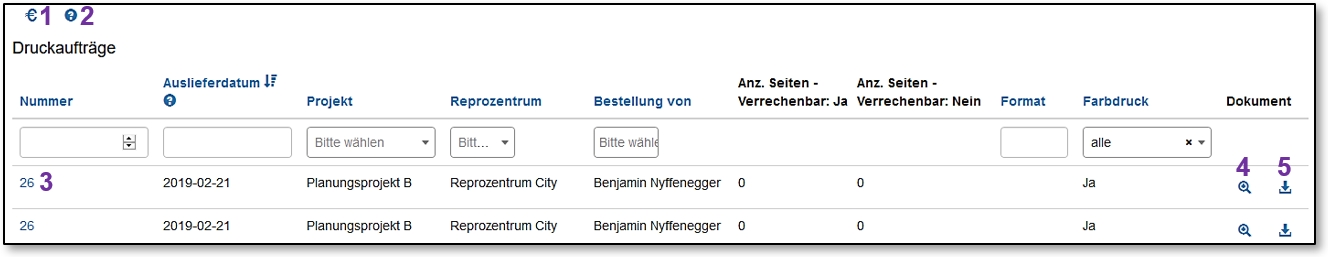
\includegraphics[width=1\linewidth]{../chapters/11_Dokumentenablage/pictures/dok_DruckauftraegeUebersicht.jpg}}
\caption{Druckauftragsübersicht}
% \label{fig:speciation}
\end{figure}

Mit Klick auf das Fragezeichen \col{(2)} erhalten Sie Infos zur Übersicht und können mit dem untenstehenden Link in die 'Dokumentenablage' wechseln:

\begin{figure}[H]
\center{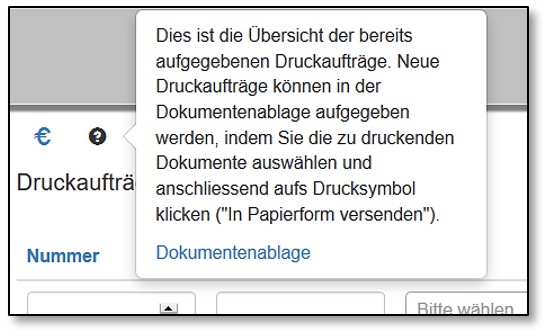
\includegraphics[width=.45\linewidth]{../chapters/11_Dokumentenablage/pictures/dok_DruckauftrInfo.jpg}}
% \caption{Neues Dokument: Zugriffsrechte}
% \label{fig:speciation}
\end{figure}

Klicken Sie auf das \euro{-Symbol} \col{(1)} erhalten Sie eine Excelliste, welche die gefilterten Druckaufträge enthält und zur Abrechnung dienlich ist:

\begin{figure}[H]
\center{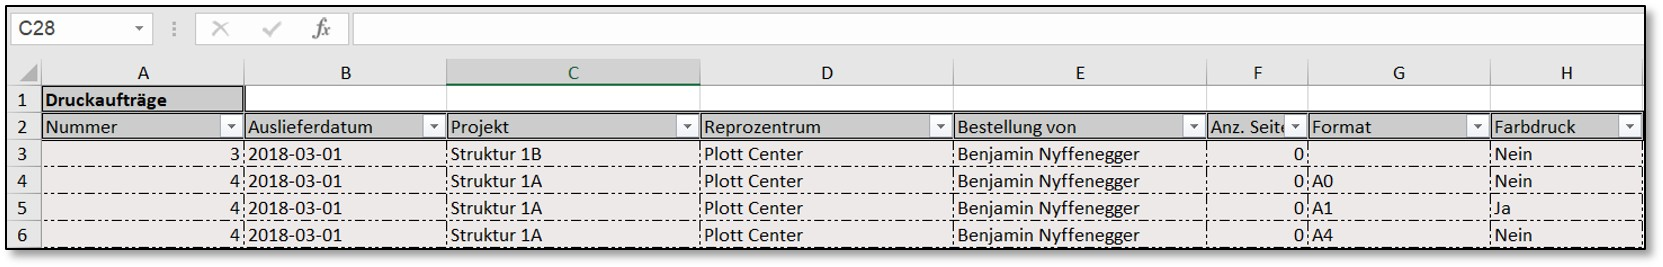
\includegraphics[width=1\linewidth]{../chapters/11_Dokumentenablage/pictures/dok_DruckauftrExcel.jpg}}
\caption{Excelexport der gefilterten Druckaufträgen}
% \label{fig:speciation}
\end{figure}

\begin{wrapfigure}[7]{l}{7cm}   % [x] Wie manche Zeile soll sich um die Grafik "brechen"
  \vspace{-25pt}      % Grundwert war 20; mit 30 schön oben beim Text ausgerichtet
  \begin{center}
    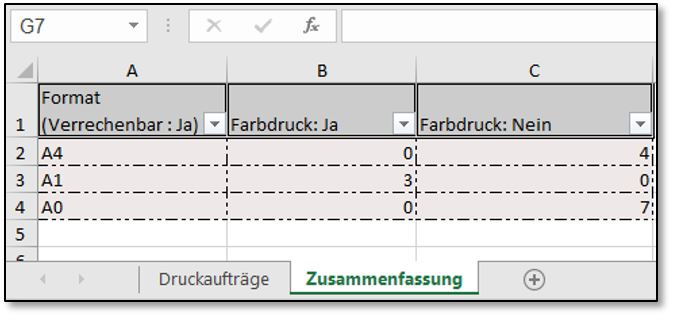
\includegraphics[width=1\linewidth]{../chapters/11_Dokumentenablage/pictures/dok_DruckauftrExcelZu.jpg}
  \end{center}
  \vspace{-20pt}
  \caption{Zusammenfassung im Excelexport}
  \vspace{-10pt}
\end{wrapfigure}

Berücksichtigt werden bei der Aufstellung die Angaben bezüglich 'Verrechenbarkeit', welche vorab in CUBE PA bei den Druckaufträgen hinterlegt wurden. Nun können Sie hier Anpassungen vornehmen und im Arbeitsblatt 'Zusammenfassung' eine Übersicht gewinnen, welche Aufträge weiter verrechnet werden können.

\vspace{1.5cm}

Mit Klick auf die Druckauftragsnummer in der Übersicht \col{(3)} erhalten Sie Detailinformationen zum Druckauftrag:

\begin{figure}[H]
\center{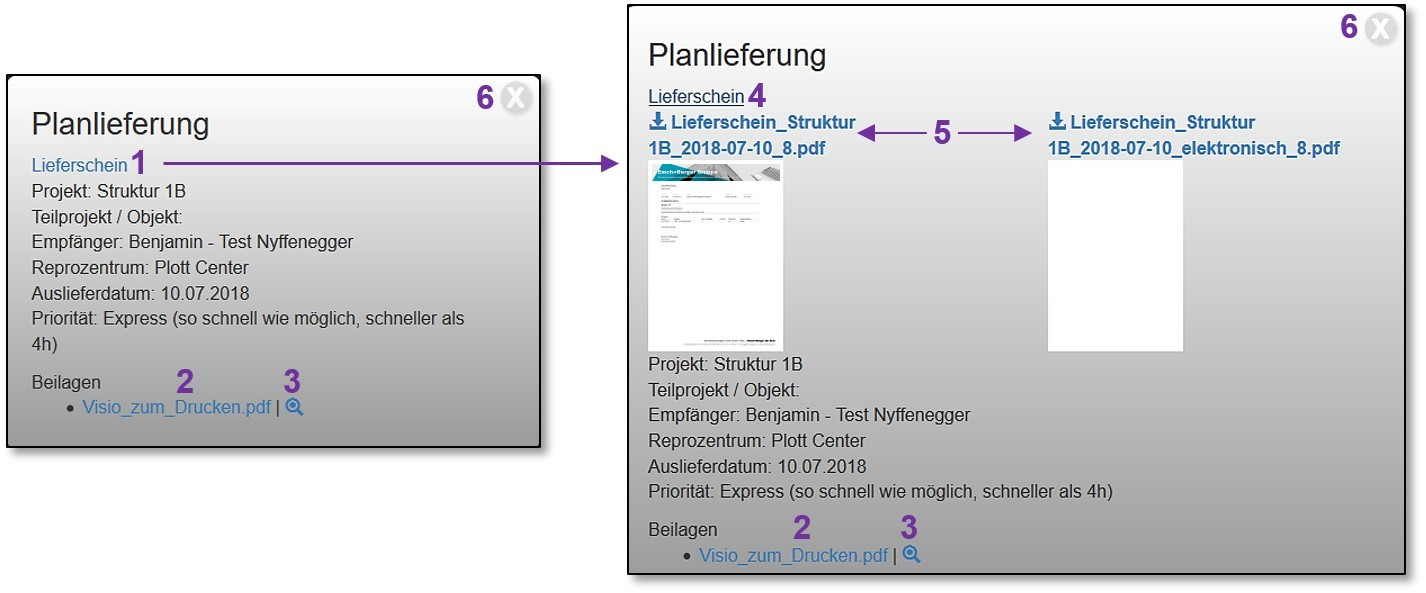
\includegraphics[width=.5\linewidth]{../chapters/11_Dokumentenablage/pictures/dok_DruckauftrDetails.jpg}}
\caption{Detailinformationen zum Druckauftrag / Lieferschein herunterladen}
% \label{fig:speciation}
\end{figure}

Mit Klick auf 'Lieferschein' \col{(1)} wird der Download-Link des Lieferscheins/der Lieferscheine eingeblendet (ZIP-Archiv) \col{(2)}. Sie können nun das ZIP-File herunterladen. Die Beilagen des Druckauftrags werden aufgelistet und mit Klick auf den Link \col{(3)} können Sie das Dokument öffnen oder speichern. Mit dem Lupensymbol 
\includegraphics[height=12pt]{/Icons/Lupe.jpg} \col{(4)} wird das Dokument in der Dokumentenablage im Betrachtungsmodus geöffnet. Mit dem 
\includegraphics[height=12pt]{/Icons/X_Button.jpg}-Button \col{(5)} verlassen Sie das Fenster wieder und kehren zur Druckauftragsübersicht.

\begin{figure}[H]
\center{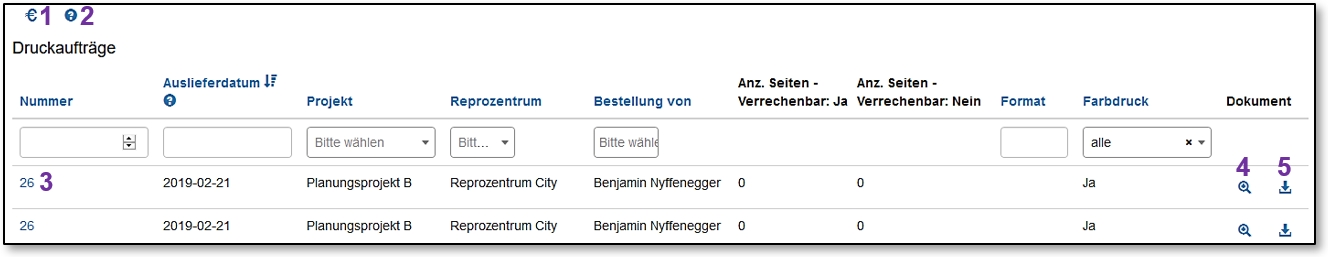
\includegraphics[width=1\linewidth]{../chapters/11_Dokumentenablage/pictures/dok_DruckauftraegeUebersicht.jpg}}
\caption{Druckauftragsübersicht}
% \label{fig:speciation}
\end{figure}

Auch von der Druckauftragsübersicht können Sie mit Klick auf das Lupensymbol 
\includegraphics[height=12pt]{/Icons/Lupe.jpg} \col{(4)} das Dokument in der Dokumentenablage öffnen (Ansichtsmodus) oder mittels dem Download-Symbol 
\includegraphics[height=12pt]{/Icons/Download.jpg} \col{(5)} das Dokument gleich öffnen oder speichern.

\vspace{\baselineskip}

\begin{wrapfigure}[13]{l}{9cm}   % [x] Wie manche Zeile soll sich um die Grafik "brechen"
  \vspace{-25pt}      % Grundwert war 20; mit 30 schön oben beim Text ausgerichtet
  \begin{center}
    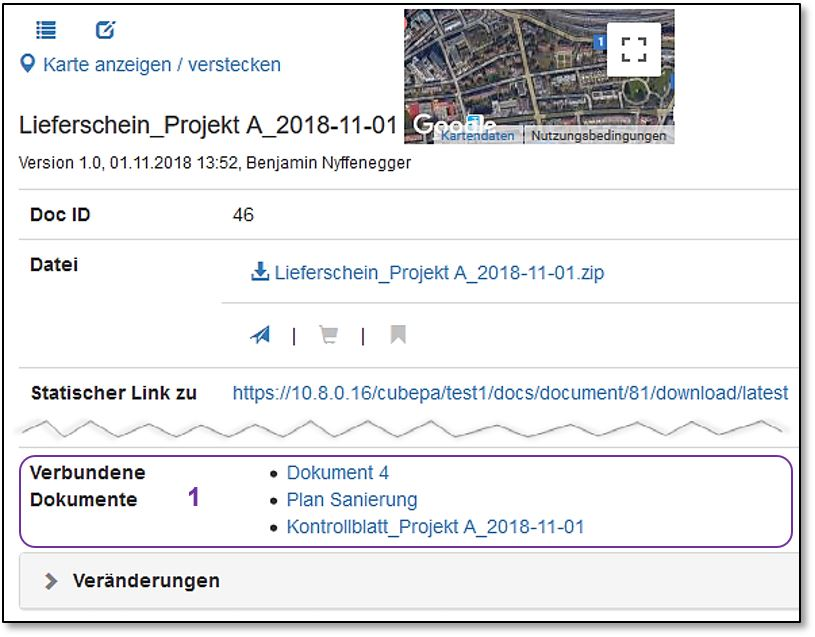
\includegraphics[width=1\linewidth]{../chapters/11_Dokumentenablage/pictures/repro_verk_Dokumente.jpg}
  \end{center}
  \vspace{-20pt}
  \caption{Verknüpfte Dokumente}
  \vspace{-10pt}
\end{wrapfigure}
Dokumente, welche beim Auftrag eines Reprodrucks erstellt worden sind (Lieferschein, Kontrollblätter), werden in der Dokumentenablage abgelegt. Im Ansichtsmodus dieser Dokumente, sowie derjenigen, welche via Reprodruck versandt wurden, sind sämtliche zusammenhängende Dokumente unter 'Verbundene Dokumente' aufgeführt \col{(1)}. Mit Klick auf den blauen Textlink gelangen Sie in den Ansichtsmodus des entsprechenden Dokuments.


\end{document}


